\documentclass[11pt, paper=a4]{scrartcl}

% CONFIG
\newcommand{\exptitle}{M\"o\ss bauer effect}       % long name of experiment 
\newcommand{\exptitleshort}{M\"o\ss bauer effect} % short name of experiment
\newcommand{\expdate}{04.04.2016}           % date of experiment
\newcommand{\exptutor}{Veronika Magerl}

% PACKAGES + MODIFICATIONS
%\usepackage[ngerman]{babel} %standard language stuff
\usepackage[T1]{fontenc}
\usepackage[utf8]{inputenc}
\usepackage{textgreek}

\usepackage{soul} %better underline
\setul{2pt}{.4pt} %set underline 2 pts below text and thickness to .4pt

\usepackage[fleqn]{amsmath}  % math
\usepackage{amssymb}

\usepackage{graphicx} %graphics
\usepackage{float} 

\usepackage[automark,headsepline]{scrlayer-scrpage} %headings
\pagestyle{scrheadings}
\ihead{\exptitleshort}
\ohead{\pagemark}
\cfoot{}

\usepackage{hyperref}
\hypersetup{
    unicode=true,          % non-Latin characters in Acrobat’s bookmarks
    pdftoolbar=true,       % show Acrobat’s toolbar?
    pdfmenubar=true,       % show Acrobat’s menu?
    pdffitwindow=false,    % window fit to page when opened
    pdfstartview={FitH},   % fits the width of the page to the window
    pdfnewwindow=true,     % links in new window
    colorlinks=true,       % false: boxed links; true: colored links
    linkcolor=blue,       % color of internal links (change box color with linkbordercolor)
    citecolor=green,       % color of links to bibliography
    filecolor=magenta,     % color of file links
    urlcolor=blue          % color of external links
}

\usepackage[labelfont=bf]{caption} % bold captions

\usepackage{chngcntr} % change behaviour of counters in different environments
\counterwithin{figure}{section}  % number figures per section
\numberwithin{equation}{section} % number equations per section
\numberwithin{table}{section}    % number tables per section

\usepackage{enumerate} % better way to config enumerates

\setcounter{tocdepth}{2} % table of contents depth

\setlength{\parindent}{0pt} % no indent on new paragraph

\usepackage{pdfpages} % include pdf files

\usepackage[nottoc,numbib]{tocbibind} % bibliography in TOC

\usepackage{isotope}
\usepackage{booktabs} %package for tables and settings
% NEW COMMANDS
\newcommand{\refeq}[1]{\overset{\text{\eqref{#1}}}{=}}

% DOCUMENT SETTINGS

\title{\exptitle}
\subtitle{}
\author{}
\date{\expdate}

% DOCUMENT
\begin{document}

\hypersetup{pageanchor=false} %stop page numbering (hyperref) to prevent for double page numers
\newcommand{\HRule}{\rule{\linewidth}{0.5mm}}
\begin{titlepage}
\begin{center}
  \textsc{\Large Fortgeschrittenen Praktikum II }\\[0.5cm]
  \HRule \\[0.4cm]
  { \huge \bfseries \exptitle}\\
  \HRule \\[0.5cm]
  \large \expdate\\[0.5cm]  
  Benjamin Winkelmann \\
  Peter Spalthoff \\
  \vspace{10pt}
  \large 
  Tutor: \exptutor \\[3cm]
  \vfill
  \normalsize
\end{center}
\end{titlepage}
\thispagestyle{empty}



\pagenumbering{Roman}
\setcounter{page}{1}


%\section*{Abstract}
In the experiment the absorption spectrum of stainless steel and natural iron are recored by using the Mössbauer effect. The Gamma radiation of a Fe-57 decay is Doppler shifted by moving the absorber relative to the source. This allows for a high relative resolution, enabling the measurement of the isometric shift in stainless steel $E_{iso}= \unit{8.61\pm0.24\cdot10^{-9}}{eV}$ and natural iron $\overline{E_{iso}} = \unit{(4.9\pm1.1)}{neV}$. Furthermore the Debye-Waller factor was calculated to be $f_s=0.51\pm0.08$.
\tableofcontents

\newpage
\listoffigures
\thispagestyle{empty}

\newpage

\listoftables

\thispagestyle{empty}

\newpage
\hypersetup{pageanchor=false} %stop page numbering (hyperref) to prevent for double page numers

\clearpage
\pagenumbering{arabic}
\setcounter{page}{1}

%physical principles
\section{Goal of the experiment}
By measuring absorption of photons of the $14.4 kev$ transition of Fe-57, in stainless steel and natural iron, the isomeric shift, the effective absorber thickness, the  Debeye-Waller-factor of the source the lifetime of the excited Fe-57 state, the magnetic field at the location of the nucleus and the magnetic moment of the $14.4 ke$V state.

\section{physical principles}
\subsection{Interaction of Gamma radiation with matter}
Photons interact with matter in three major ways\cite{Demtröder}:
\paragraph{Photoelectric effect} \ \\
Shell electrons of atoms absorb photons and gain its energy, leaving the potential well of the atom and exiting the shell with the energy $E_e = E_\gamma-E_B$ with $E_B$ being the binding energy of the electron.
\paragraph{Compton scattering} \ \\
Compton Scattering is the elastic scattering of photons at quasi free  electrons ($E_B << E_\gamma$) and its wavelength $\lambda=2\pi c/\omega$ is shifted, depending on the scattering angle $\varphi$(see figure \ref*{eq:compton}):
\begin{equation}
\lambda_S -\lambda_0 = \frac{2 \pi \hbar}{m_e c}(1-cos(\varphi))
\label{eq:compton}
\end{equation}
\paragraph{Pair Production} \ \\
A photon can produce a positron electron pair if it has an energy of at least $2\cdot m_e=1.022MeV$ the photon is lost in the processes reducing the Intensity of the photon beam.\\ \ \\
Due to those processes the intensity of electromagnetic radiation decreases exponentially with penetration depth $d$:
\begin{equation}
I(d)=I_0 \cdot exp(-\mu d)
\end{equation}
where $\mu$ is the attenuation coefficient.
\begin{figure}[h]
	\centering
	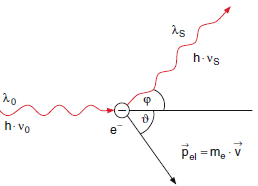
\includegraphics[width=0.5\linewidth]{graphics/Compton}
	\caption[Compton scattering]{Compton effect: A photon is scattered by a (quasi) free electron changing its direction by an angle $\varphi$\cite{Demtröder} }
	\label{fig:principles:Compton}
\end{figure}

\begin{figure}[H]
	\centering
	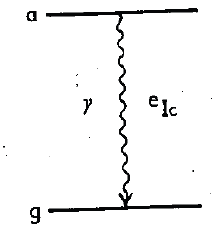
\includegraphics[height=0.18\textheight]{graphics/Emission}
	\caption[spontaneous $\gamma$ emission]{principle of spontaneous $\gamma$ emission of excited nuclei. Transitioning from an excited state ($E_a$) to the ground state ($E_g$) the nucleus emits a photon with energy $E_a-E_g=\hbar\dot \omega$ or transmits that energy directly to an electron of the atomic shell.\cite{Wegener}}
	\label{fig:principles:Emission}
\end{figure}
\subsection{Gamma Decay and resonance absorption}
Nuclei in excited states (energy $E_a$) can spontaneously transition into the ground (energy $E_g$) state. The energy $\Delta E$ the nucleus loses is either carried by an emitted photon (spontaneous emission) or directly gained by a shell electron (inner conversion). \\
In the case of spontaneous emission, the photon can be absorbed by a nucleus of the same kind which thereby transits into an excited state. This is called resonance absorption. However due to the recoil the nuclei receive this rarely happens for free atoms.
Consider the rest frame of a nucleus, that means its momentum is $p_0 = 0$. Now consider this nucleus decays by emitting a photon. Since the photon carries the momentum 
\begin{equation}
 p = \frac{E_\gamma}{c}= \frac{\hbar}{c}\cdot \omega
\label{eq:momentum}
\end{equation}
with the reduced Planck constant $\hbar$ and c the speed of light, and momentum is conserved the nucleus receives a recoil equal to the photons momentum and therefore also kinetic energy or recoil energy $R$. The emitted photon therefore has the energy \cite{Eyges}:
\begin{equation}
E_\gamma=\Delta E - \frac{p^2}{2m} = \Delta E - \frac{(\hbar \omega)^2}{2mc^2} =:\Delta E-R
\label{eq:recoil:emission}
\end{equation}
When the photon is absorbed the same applies: the absorbing nucleus receives the recoil $R$. This means for a photon to be absorbed, inducing a nuclear transition with $\Delta E$ the photon has to have the energy:
\begin{equation}
E_\gamma=\Delta E + R
\label{eq:recoil:absorbtion}
\end{equation}
In consequence the absorption spectrum is shifted relative to the emission spectrum (see fig \ref{fig:principles:lorentz} depending on the recoil energy $R$.

\begin{figure}[hpbt]
	\centering
	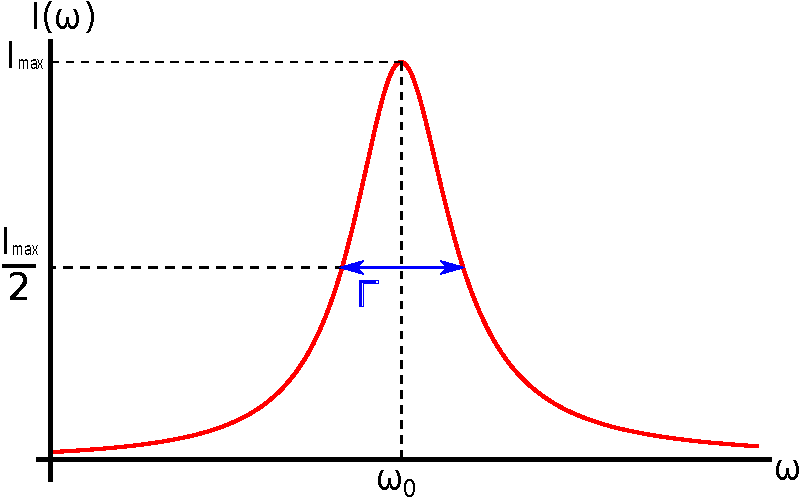
\includegraphics[height=0.25\textheight]{graphics/Lorentz.pdf}
	\caption[Lorentz distribution]{Lorentz distribution: $I(\omega) \propto \frac{1}{(\omega-\omega_0)^2+(\Gamma /2)^2}$\\}
	\label{fig:principles:lorentz}
\end{figure}

\subsection{Doppler shift}
Due to thermal motion the emitting nucleus and the absorbing nucleus have relative velocity $v$, shifting the frequency via Doppler effect:  
\begin{equation}
E_\gamma^{'} = E_\gamma (1+\frac{v}{c}) 
\label{eq:doppler shift}
\end{equation}
So the energy is changed by:
\begin{equation}
E_\gamma^{'} - E_\gamma = E_\gamma \frac{v}{c}
\label{eq:diffdopplershift}
\end{equation}


\subsection{Mößbauer effect}
The Mößbauer effect is the name for the phenomenon of \emph{recoilless emission} (or absorption). Revisiting equation \ref{eq:recoil:emission} one an see that the recoil energy $R=\frac{(\hbar \omega)^2}{2mc^2}$ is inversely proportional to the mass of the nucleus. In a solid it is possible for the whole lattice the absorb the recoil therefore increasing the recoiled mass enormously, so that $R\approx0$\footnote{this is a simplified description, for a more detailed one see \cite{Eyges} and \cite{Wegener} }. This effect means atoms that shows this behavior (In this experiment Fe-57) can emit photons, that can be reabsorbed by atoms of the same kind.

%\subsubsection{Einstein lattice}
%In the Einstein model the atoms of a lattice are described as three dimensional quantum mechanical oscillators, all with the same frequency $\omega_E$ This means the lattice can only increase its energy in quanta of $\hbar \omega_E$ so if $E_\gamma < \hbar \omega_E$ the absorption is recoilless.
%\subsubsection{Debye mdoel}
%In contrast to Einstein's model, this model allows for several frequencies, introducing a dispersion relation for the vibrational spectrum:
%\begin{equation}
%\omega = c_S\cdot k
%\end{equation}
%Where $c_S$ is the speed of the sound and k is the wave vector 
\subsection{Debye-Waller factor}
The Debye-Waller factor is the ratio of recoilless absorption.
\begin{equation}
f = exp \left[ -\frac{3R}{2k \cdot \Theta_D} \left(1+ \frac{4T^2}{\Theta_D^2}\int_{0}^{\Theta/T}\frac{xdx}{e^x-1}\right) \right]
\end{equation}
Where $R$ is the recoil energy, $k$ the Boltzmann constant, $\Theta_D$ the Debye temperature. 
If the temperature is low $T<<\Theta_D$ this can be simplified to:
\begin{equation}
f \approx exp\left[ -\frac{3R}{k \cdot \Theta_D} \left( \frac{3}{2}+\frac{\pi^2 T^2}{\Theta_D^2}\right) \right]
\end{equation}

\begin{figure}
\centering
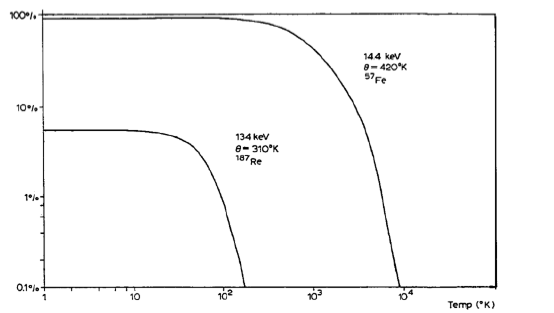
\includegraphics[width=0.7\linewidth]{graphics/Debeyfactor}
\caption[Debey factors]{Debye factor as a function of temperature in Fe-57 and Re-187. At room temperature Fe-57 has a ratio of recoilless emission absorption of 0.91}
\label{fig:principles:Debeyfactor}
\end{figure}

\subsection{Isomer shift}
Since electrons of an atomic shell are kept within the coulomb potential of the nucleus their potential energy depends on the charge distribution in the nucleus. Transitioning to an excited state affects this distribution therefore also affecting the potential energy of the electrons. This change in energy shifts the frequency that an absorbed photon must have to induce the transition\cite{Wegener}.
\subsection{Hyperfine splitting}
The nucleus has magnetic moment ($\mu_I$) and spin $I$. In a surrounding magnetic field $H$ the energy level splits into $2I+1$ sub-energy levels. The sub-sates are characterized by the magnetic quantum number $m_I = -I,I+1..,I-1,I$ and the energy difference induced is:
\begin{equation}
E_{HFS}=\frac{\mu_I m_I H}{I}
\end{equation}
\begin{figure}[H]
\centering
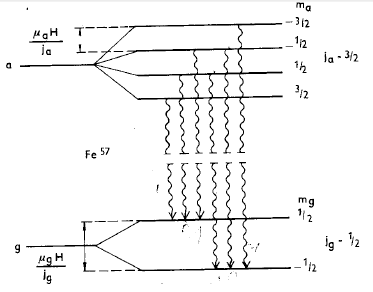
\includegraphics[width=0.5\linewidth]{graphics/HFS}
\caption[Hyperfine splitting Fe-57]{Hyperfine splitting for Fe-57 in magnetic field H for the ground state g ($I_g = 1/2$) and the excited state ($I_a=3/2$).\cite{Wegener}}
\label{fig:HFS}
\end{figure}
The transition $m_a \rightarrow m_g$ emits photons with energy $\omega$:
\begin{equation}
E_\gamma(m_a,m_g) = E_0 - \left( \frac{\mu_a m_a}{I_a}-\frac{\mu_g m_g}{I_g}\right) H
\label{eq:HFS}
\end{equation}




\section{Experimental setup}
\subsection{Method}
To measure the absorption spectra of stainless steel and natural iron, we irradiate the samples with the $14.4keV$ $\gamma$-radiation emitted by a radioactive source. To vary the frequency a motor is used to move the absorber relative to the source (Doppler shift see  \ref{eq:diffdopplershift}). By repeating this measurement for different absorber velocities a spectrum is recorded.\\
\subsection{Setup}
\begin{figure}[hbt]
\centering
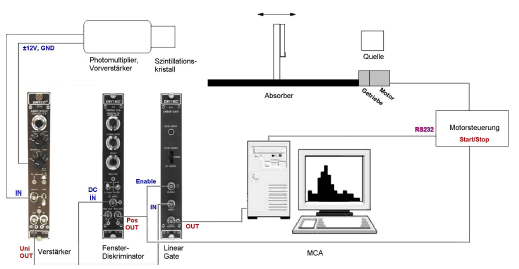
\includegraphics[width=1.0\linewidth]{graphics/Aufbau}
\caption[Setup overview ]{Overview of the experimental setup}
\label{fig:Aufbau}
\end{figure}

The setup consists of the $\gamma$ source, the absorber on a track, the motor used to move the absorber at constant speeds relative to the source and as the photon detector a scintillator is used. The light signal of the scintillator turned into an electric signal by a photomultiplier. This signal is amplified and shaped in the amplifier. The amplifier has two exits, one of which is connected to a single channel analyzer (SCA). If the signal pulse is within an adjustable window the SCA sends a standardized signal and enables the linear gate, which is also connected to the amplifier via a delay to ensure simultaneity of the signals. If the linear gate is enabled when it receives a signal from the amplifier it transmits the amplifier signal to the multichannel analyzer (MCA), which is read out with a Computer. The second output of the SCA is connected to a counter, which also can be read out with the Computer.

\subsection{The source Co-57}
\isotope[57]{Co} decays via electron capture with a branching ratio of $99.8 \%$ and a half life of 270d into an iron in an excited state $\isotope[57]{Fe^*}$. This state decays with a half life of 9ns an branching ratio of $88\%$ into the $14.4keV$ excited state which finally decays to the ground state (Branching ratio for $\gamma-decay$ is $10\%$) \ref{fig:principles:Zerfallsschema2}. 
\begin{figure}[hbt]
	\centering
	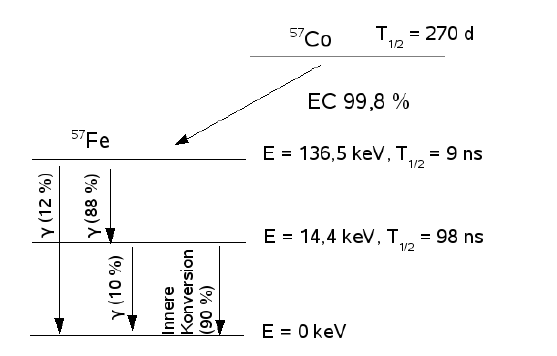
\includegraphics[width=0.5\linewidth]{graphics/Zerfallsschema2}
	\caption[Co-57 decay]{decay series of Cobalt-57}
	\label{fig:principles:Zerfallsschema2}
\end{figure}
\subsection{Procedure}
\subsubsection{MCA calibration}
To calibrate the MCA the spectra of Cu, Rb, Mo, Ag, Ba, and Tb are measured for 300s each. For the Cu no peak
\subsubsection{background measurement}


\section{Analysis}
\subsection{Identifying the Fe-57 transition peak}
\begin{figure}[H]
\centering
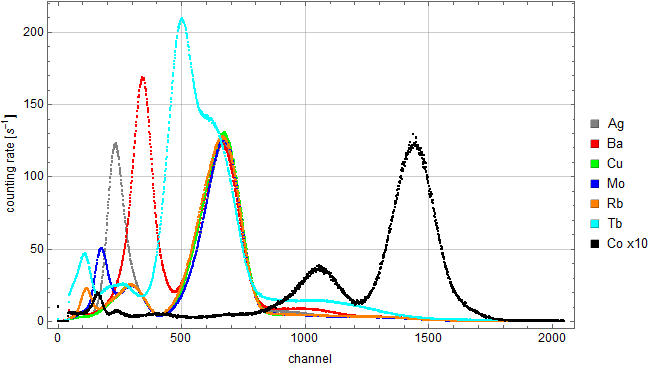
\includegraphics[width=1\linewidth]{../results/calibration/spectra}
\caption[Reference spectra]{Plot of all recorded reference spectra and the cobalt source (upscaled by factor 10 for better comparability)}
\label{fig:analysis:spectra}
\end{figure}
Around channel 700 all target samples have clearly defined peak. For Terbium(Tb) this peaks blends with its $K$-line. This peak is caused by photons of the americium source, passing through the targets without interacting. The $K_\alpha$-line of copper (Cu) is beyond the left edge and therefore not meassured. The peak positions are estimated from the fig \ref{fig:analysis:spectra}. The error is estimated to be $s_{Ch}=10$. The Result can be seen in table \ref{tb:analysis:peakpos}. One can already identify the peak since it has to lie between the Rb-peak and the Mo-peak, which is suggesting the peak furthest to the left (around channel 160) belongs to the 14.4keV line.

\begin{table}[H]\centering
	\begin{tabular}{@{}llllll@{}}
		\toprule
		 traget & energy [keV]& peak channel  \\
		\midrule
		Cu & 8.04 & - \\
		Rb & 13.37 & 120 \\
		Mo & 17.44 & 180 \\
		Ag & 22.10 & 230 \\
		Ba & 32.06 & 340 \\
		Tb & 44.23 & 500\\
		\bottomrule
	\end{tabular}
	\caption[peak positions]{number of the channel for the $K$-line peaks}
	\label{tb:analysis:peakpos}
\end{table}

The Linear function $E(ch)=a\cdot ch+b$ was fitted to the data see figure
\begin{figure}[H]
\centering
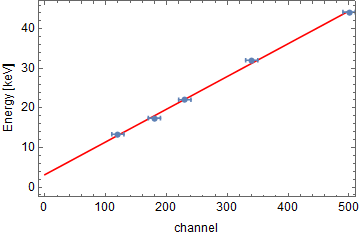
\includegraphics[width=1.0\linewidth]{../results/calibration/fit}
\caption[MCA calibration]{Linear fit for the calibration of the MCA}
\label{fig:calibrationfit}
\end{figure}
The results are:
\begin{equation}
\begin{aligned}
	a &= (0.083\pm0.002)keV\\
	b &= (3.2 \pm 0.6)keV
\end{aligned}
\end{equation}
The position of the 14.4keV peak should be at\footnote{error calculated according to gaussian error propagation. Unless specified otherwise, all errors of values calculated with other values are determined this way}:
\begin{equation}
ch_{14.4keV}=\frac{14.4keV-b}{a}=135\pm4
\end{equation}
A Comparison with figure \ref{fig:analysis:spectra} shows that the peak furthest to left is the closest ($ch=160\pm10$)to this value, however the values lie more almost two standard deviations apart. Fortunately, an exact calibration is not needed for further analysis.
\subsection{Compton}
High energy photons such as those from the transitions with \unit{122}{keV} and \unit{136}{keV} lose energy when passing through matter via the Compton effect. Some of these photons will randomly fall within the energy windows that was set for the measurements and thus pose an underground that needs to be subtracted from the data for parts of the further analysis. Since higher energy photons lose their energy slower than lower energy photons when passing through matter, one can separate the two by placing aluminum plates in the beam with a range of thicknesses. The count rate decreases exponentially with the thickness $d$ 
\begin{equation}
\dot{N}=\dot{N}_0e^{-\mu d}
\end{equation}
measurements were taken for absorber thicknesses between $d=\unit{0.21}{mm}$ and $d=\unit{12.43}{mm}$, which were measured with a caliper to such high precision that the error is far smaller than the Poisson error on the count rates and is thus neglected. Figure \ref{fig:comptonbackground} shows the measured data.
\begin{figure}
\centering
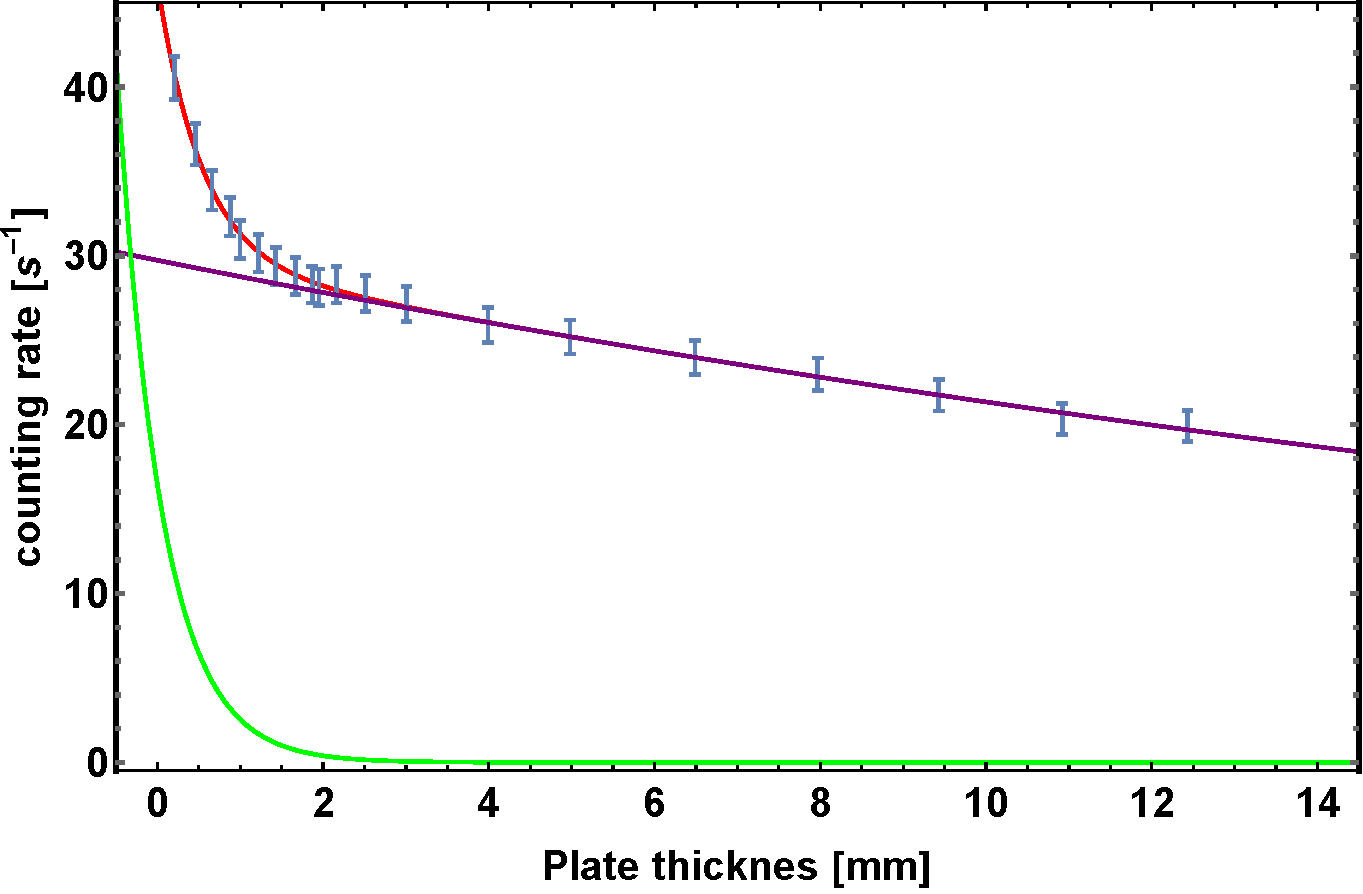
\includegraphics[width=1.0\linewidth]{graphics/comptonbackground}
\caption[Compton background data]{The compton background data along with the fitted sum of the two exponential functions in red. The curve for Compton underground is colored purple and that for the \unit{14,4}{keV} photons green.}
\label{fig:comptonbackground}
\end{figure}
As two processes with different speeds, $\mu_{C}$ of the Compton background and $\mu_0$ of the actual data, are expected, the fit function for the count rates for varying absorbers is
\begin{equation}
\dot{N}(d)=A_C\cdot e^{-\mu_C d}+A_0\cdot e^{-\mu_0 d}
\end{equation}
The resulting fit parameters for the Compton underground were
\begin{align}
A_C&=\unit{(29.74\pm0.17)}{s^{-1}}\\
\mu_C&=\unit{(0.0331\pm0.0009)}{mm^{-1}}
\end{align}
As no aluminum plates are used during regular measurements, the value for $d=0$, and thus the fit parameter $A_C$, is the underground rate to be deducted from future measurements.

\subsection{Attenuation of the acrylic glass}
The acrylic glass in which the sample is cased absorbs some of the radiation. To quantify this, a plate of acrylic glass of roughly the same thickness as the one used to case the sample can be but into the beam. One measurement is taken with the plate and one without. The thickness of the plate was measured as $d=\unit{(1.94\pm0.01)}{mm}$. The resulting count rates were
\begin{align}
\dot{N}_0&=\unit{(107.4\pm0.3)}{s^{-1}}\\
\dot{N}_A&=\unit{(84.8\pm0.3)}{s^{-1}}
\end{align}
where the uncertainties stem from the Poisson errors on the number of counts. With the values given for the attenuation coefficient $\mu/\rho=\unit{1.101}{cm^2/g}$ and the density of the acrylic glass $\rho=\unit{1.19}{g/cm^3}$ in \cite{anleitung}, the mass attenuation coefficient $\mu=\unit{1.31019}{1/cm}$ can be calculated. With this value as well as the thickness of the plate, the count rate after the acrylic glass can also directly be calculated from the count rate without the acrylic glass as
\begin{equation}
\dot{N}_A^{calc}=\dot{N}_0\cdot e^{-\mu d}=\unit{(83.3\pm0.3)}{s^{-1}}
\end{equation}
The two values agree only with their $2\sigma$ intervals. The literature value $\mu/\rho=\unit{1.101}{cm^2/g}$ is actually listed for energies of $E_\gamma=\unit{15}{keV}$, which is slightly more than the that of the $\unit{14.4}{keV}$ transition. However, the value is higher for lower energies, which means that using a value for the exact energies of the photons in this experiment would lead to an even lower calculated count rate. The likely cause for the disagreement of the values is thus likely that the thicknesses of the plates do no match. A quick calculation reveals that a disagreement of 5\% would bridge the gap and have the values agree within their $1\sigma$ intervals.
\subsection{Single line absorber}
The results for the measurement of the absorption spectrum of stainless steel can be seen in figure \ref{fig:single line absorber:fitresult}. To evaluate the data a voigt function (convolution of a Gaussian and Lorentz) was fitted to it:
\begin{equation}
f(v)=B- A \cdot Voigt((v-v_0),\delta,\sigma )
\end{equation}
where $v$ is the absorber velocity, $v_0$ the peak position, $\delta$ is the 
\begin{figure}[H]
\centering
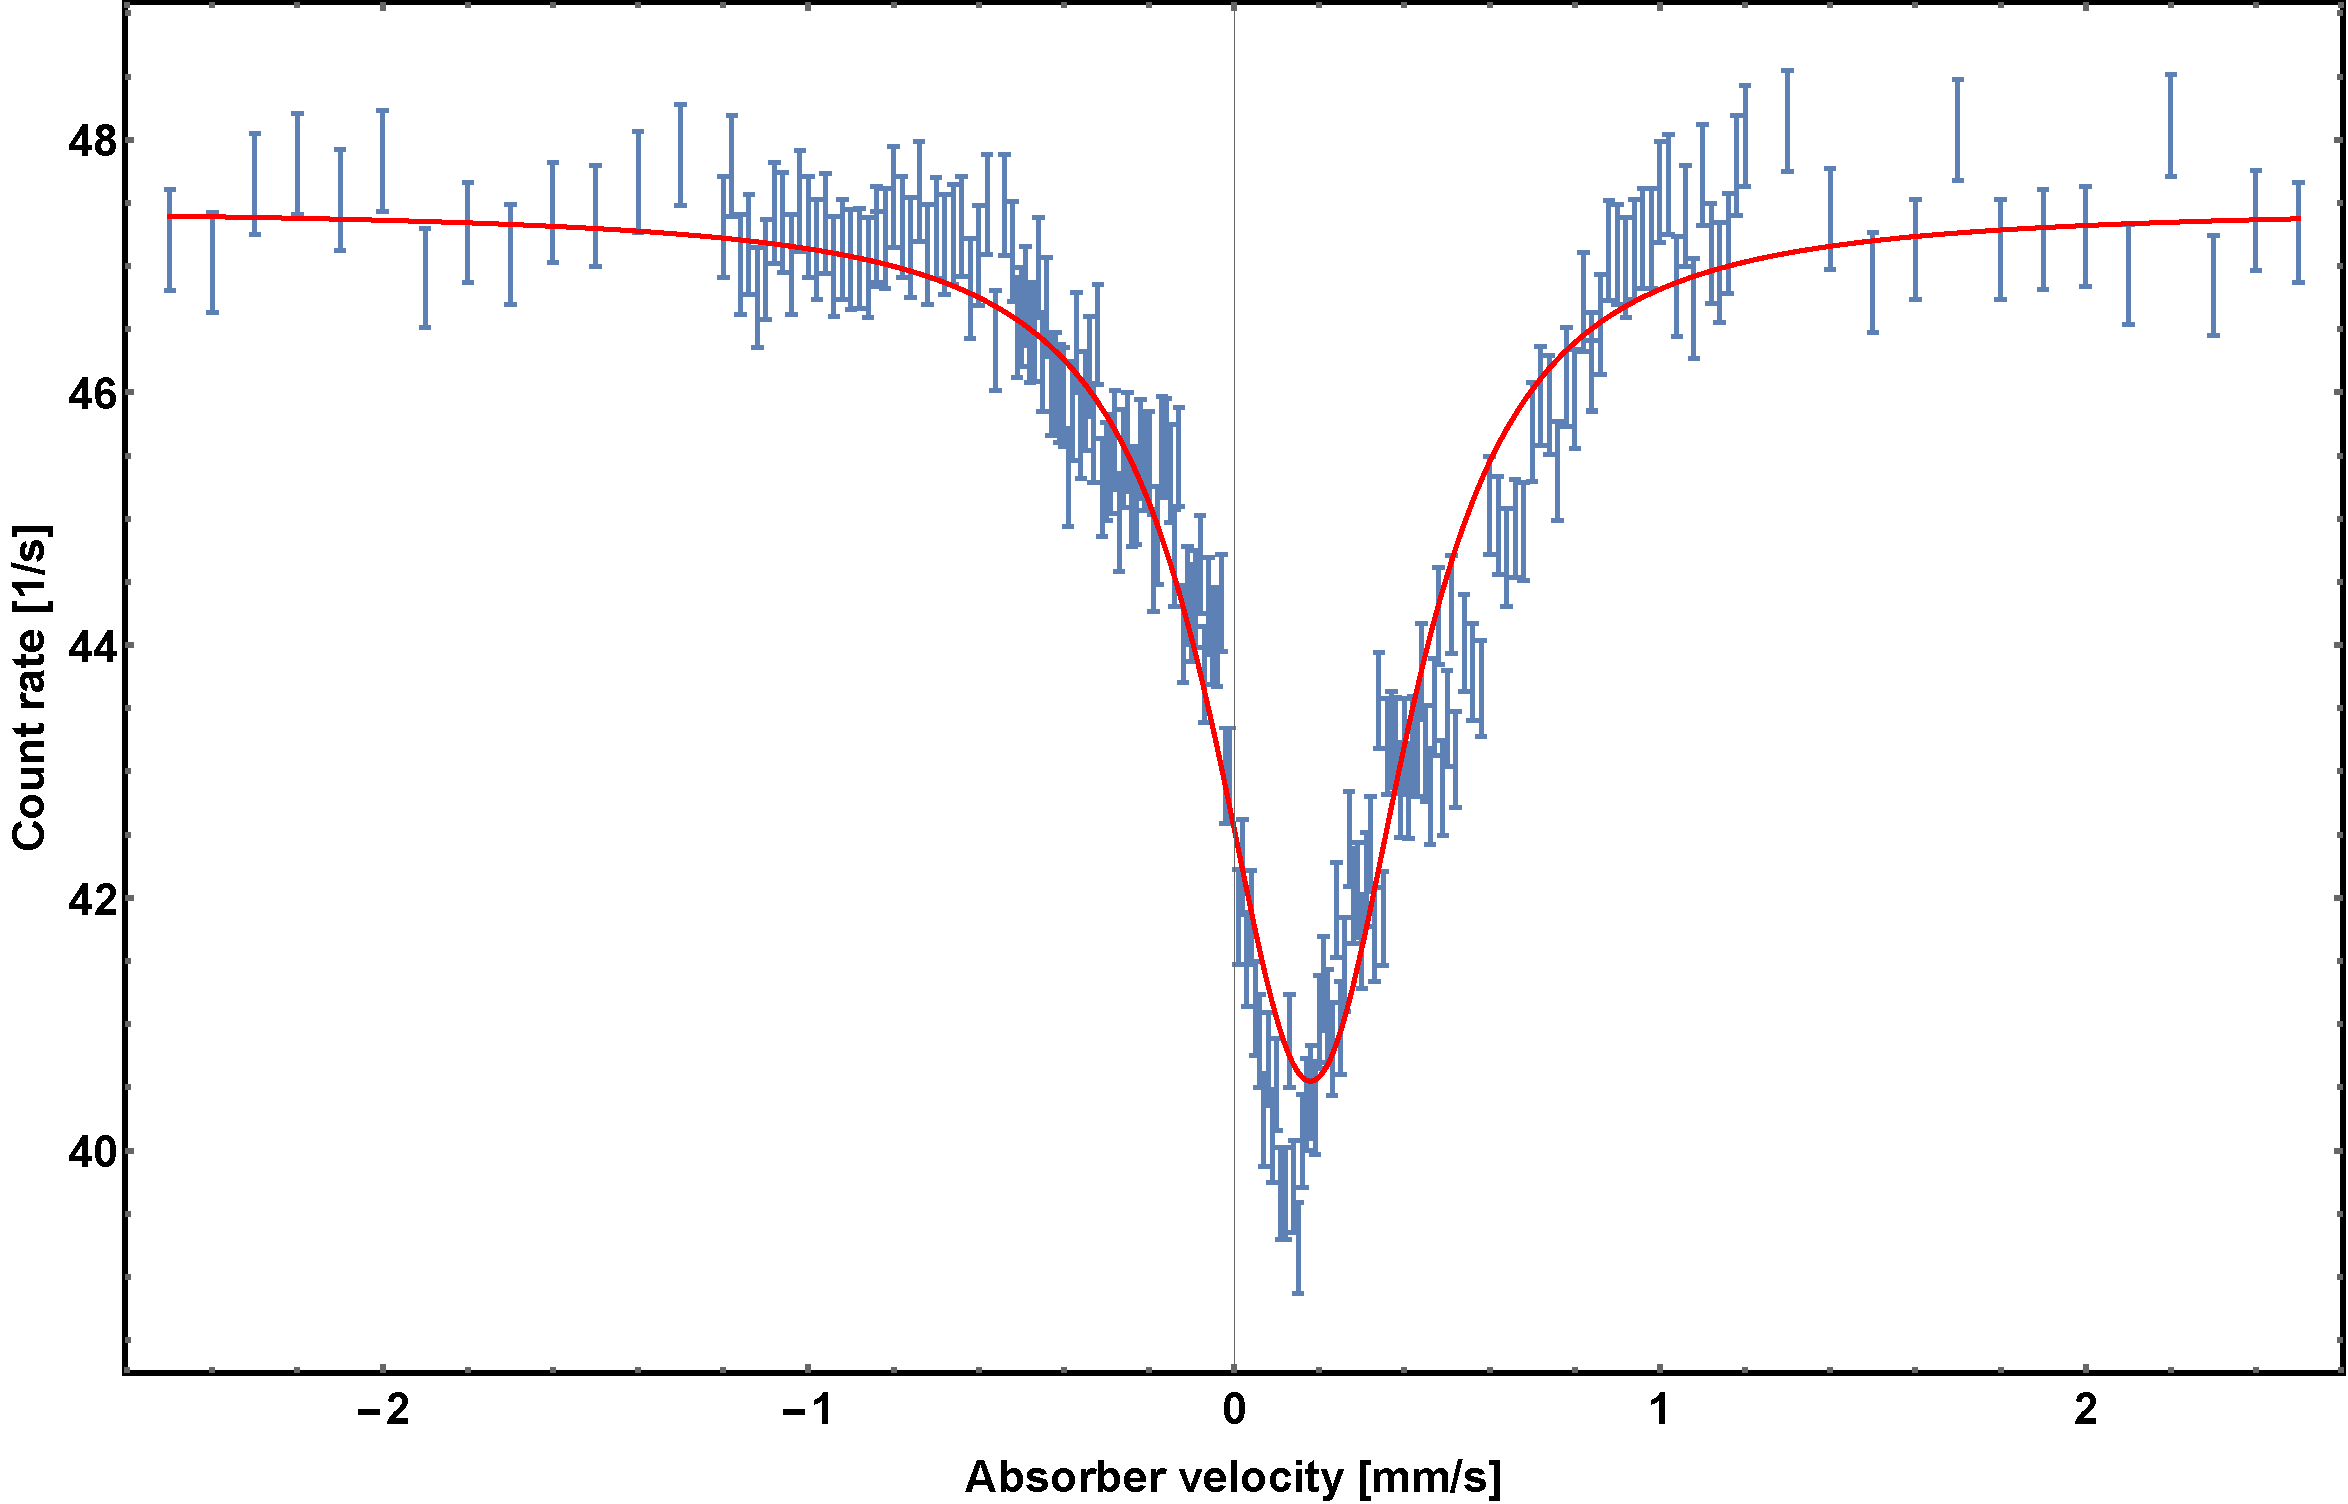
\includegraphics[width=1.0\linewidth]{../results/steel/voigtfittry.pdf}
\caption[Stainless steel spectrum]{Measured absorption spectrum for stainless steel and Voigt fit.}
\label{fig:single line absorber:fitresult}
\end{figure}
The fit results are:\\ \ \\
$\begin{array}{l|llll}
\text{} & \text{Estimate} & \text{Standard Error} \\
\hline
v_0 & 0.179 & 0.005\\
\sigma  & 0.25 & 0.03 \\
\delta  & 0.14 & 0.10\\
\text{B} & 47.46 & 0.11\\
A & 5.8 & 0.4 &\\
\end{array}$

\subsubsection{Isomeric shift} \ \\
Since the background is constant it only effects variable $B$ of the fit function, therefore
with the parameter $v_0$ one can calculate the isomeric shift, without having to correct for the background. \ref{eq:diffdopplershift}:
\begin{equation}
E_{iso} = (8.614\pm0.24)\cdot 10^{-9} eV
\end{equation}
\subsubsection{Effective absorber thickness}
\label{sec:effab}
 \ \\
The effective absorber thickness is given by \cite{anleitung}:
\begin{equation}
T_A = f_An_A\beta\sigma_0d_A
\label{eq:effective absorber thickness}
\end{equation}
where $d_A = 25\mu m$ is the absorber thickness, $n_A$ is the number of iron atoms per volume, $\beta=0.022$ the ratio of Fe-57 in the isotope mixture, $\sigma_0$ the cross section and $f_A=0.8$ the Debye-Waller-factor of the absorber.
To calculate $n_A$ literature values are used (\cite{webelements}):

\begin{equation*}
\begin{aligned}
N_A &= 6.022 \cdot 10^{23} mol^{-1} \qquad& \text{Avogadro constant}\\
\rho_{Fe} &= 7.874 g/cm^3 \qquad& \text{density of iron} \\
A_Fe &= 55.845 g/mol \qquad& \text{molar mass of iron}\\
r &=  (0.70\pm0.05) \qquad& \text{fraction of iron in the absorber\cite{anleitung}}
\end{aligned}
\end{equation*}
The number of Fe atoms per volume is then given by:
\begin{equation*}
\frac{\rho_{Fe}}{A_Fe}N_A\cdot r= (5.9\pm0.4)\cdot 10^{22} cm^{-3}
\end{equation*}
The absorption cross section is given by \cite{Wegener}:
\begin{equation}
\sigma_0= \frac{\lambda^2}{2\pi} \left(\frac{2I^*+1}{2I+1}\right) \frac{1}{1+\alpha}
\end{equation}
where $\alpha =9$ (see \cite{Wegener}) is the conversion coefficient, $\lambda$ the wavelength of the absorbed photon, $I^*=3/2$ and $I=1/2$  are the nuclear spins of the excited and ground state. With $\lambda = \frac{hc}{E_\gamma}=86.14 pm$, the cross section is:
\begin{equation}
\sigma_0=2.36\cdot 10^-22m^2
\end{equation}
Plugging those values in equation \ref{eq:effective absorber thickness}, the effective absorber thickness is:
\begin{equation}
T_A = (6.2\pm 0.4)
\end{equation}
\subsubsection{Debye Waller factor of the source}
The Debye-Waller-factor is related to the count rate with no absorption $Z(\infty)$, the minimal count rate $Z(v_min)$ (maximal absorption) and the effective absorber thickness $T_A$ \cite{Wegener}:
\begin{equation}
\frac{Z(\infty)-Z(v_{min})}{Z(\infty)}=f\cdot [1-exp(-\frac{T_A}{2})J_0(\frac{iT_A}{2})]
\label{eq:debye}
\end{equation}
$i$ is the imaginary unit and $J_0$ the order zero Bessel function. The count rates on the left can be determined from the fit function $f(v)$ and the Compton background $A_C$:
\begin{equation}
\begin{aligned}
Z(\infty) &= B - A_C\\
Z(v_{min}) &= A-A_C\\
\end{aligned}
\end{equation}
Rearranging equation \ref{eq:debye} we get for the Debye-Waller factor of the source
\begin{equation}
f_s= 0.51\pm0.08
\end{equation}
The rather big error ($15\%$) is mainly caused by the uncertainty of $Z(v_{min})$ since all errors of the fit function parameters contribute.

\subsubsection{life time of the 14.4keV state}
\paragraph{From the fit}\ \\
From the Voigt fit the half width $\delta = 0.14 \pm 0.10$ of the convoluted Lorentzian can be extracted. It has to be noted, that $\delta$ from the fit is still in units of velocity (mm/s), so using equation \ref{eq:diffdopplershift} the wanted half width $\Gamma$ is:
\begin{equation}
\Gamma  = 6.2\pm4.6\cdot 10^{-8} eV
\end{equation}
With Heisenberg's uncertainty relation $\Gamma \cdot \scalebox{1.5}{$\tau$}=\hbar$, the mean life time is:
\begin{equation}
\scalebox{1.5}{$\tau$}= (11\pm8)ns
\end{equation}
The fit uncertainty propagates through the calculation and is responsible for the 
relative error of over $70\%$. Despite of this the literature value \scalebox{1.5}{$\tau$}$_{lit}$=141ns is still more than seven standard deviations away from the determined value.

\paragraph{From the effective absorber thickness} \ \\
The relative line broadening $\Gamma_a/2\Gamma$ is determined graphically from figure \ref{fig:absorberthicknessevaluated}. For this purpose the program Inkscape was used. By measuring the length of each coordinate axes in pixels, factors are determined, allowing the conversion between line lengths in pixels and their corresponding values.\\
\begin{figure}[hbp]
	\centering
	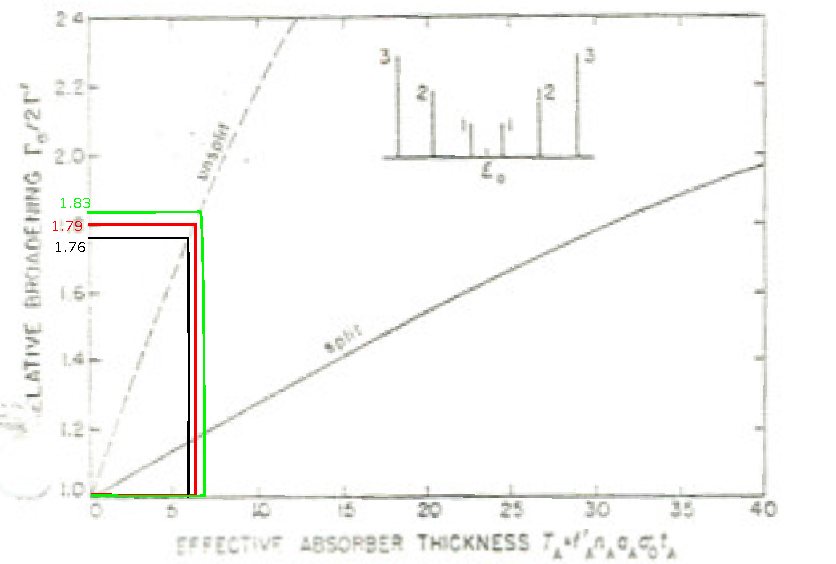
\includegraphics[width=1.0\linewidth]{graphics/absorberthicknessevaluated}
	\caption{Graphical determination of the relative line broadening\cite{Frauenfelder}}
	\label{fig:absorberthicknessevaluated}
\end{figure}
The effective absorber thickness was calculated in section \ref{sec:effab}. To estimate the error, the relative broadening was also determined for $T_A\pm s_{T_A}$. The results are:
\begin{table}[H]\centering
	\begin{tabular}{@{}llllll@{}}
		\toprule
		$T_A$ & $\frac{\Gamma_a}{2\Gamma}$ \\
		\midrule
		5.8 & 1.76\\
		6.2 & 1.79 \\
		6.6 & 1.83 \\
	\end{tabular}
	\caption[relative broadening]{relative broadening for different absorber thicknesses}
	\label{tb:relative broadening}
\end{table}
For the error estimation the bigger difference (0.04) is chosen. As the peak width of the absorber, the width of the fitted Voigt profile is used, calculated with an empirical  approximation($0.02\%$ accuracy)\cite{Olivero}:
\begin{equation}
\Gamma_a=0.5*(1.0692\cdot \delta+\sqrt{0.86639\cdot \delta^2 + 4\cdot (2\sigma\sqrt{2ln(2)})})
\end{equation}
and with the values from the Voigt fit for $\delta$ and $\sigma$
\begin{equation}
\Gamma_a=(32\pm4)*neV
\end{equation}
and
\begin{equation}
\Gamma=(8.9\pm0.6)neV
\end{equation}
Due to the time-energy uncertainty the mean life time is then given by:
\begin{equation}
\scalebox{1.5}{$\tau$}=\hbar/\Gamma=()6.5\pm0.4)ns
\end{equation}

\subsection{Six-line absorber}

\begin{figure}
\centering
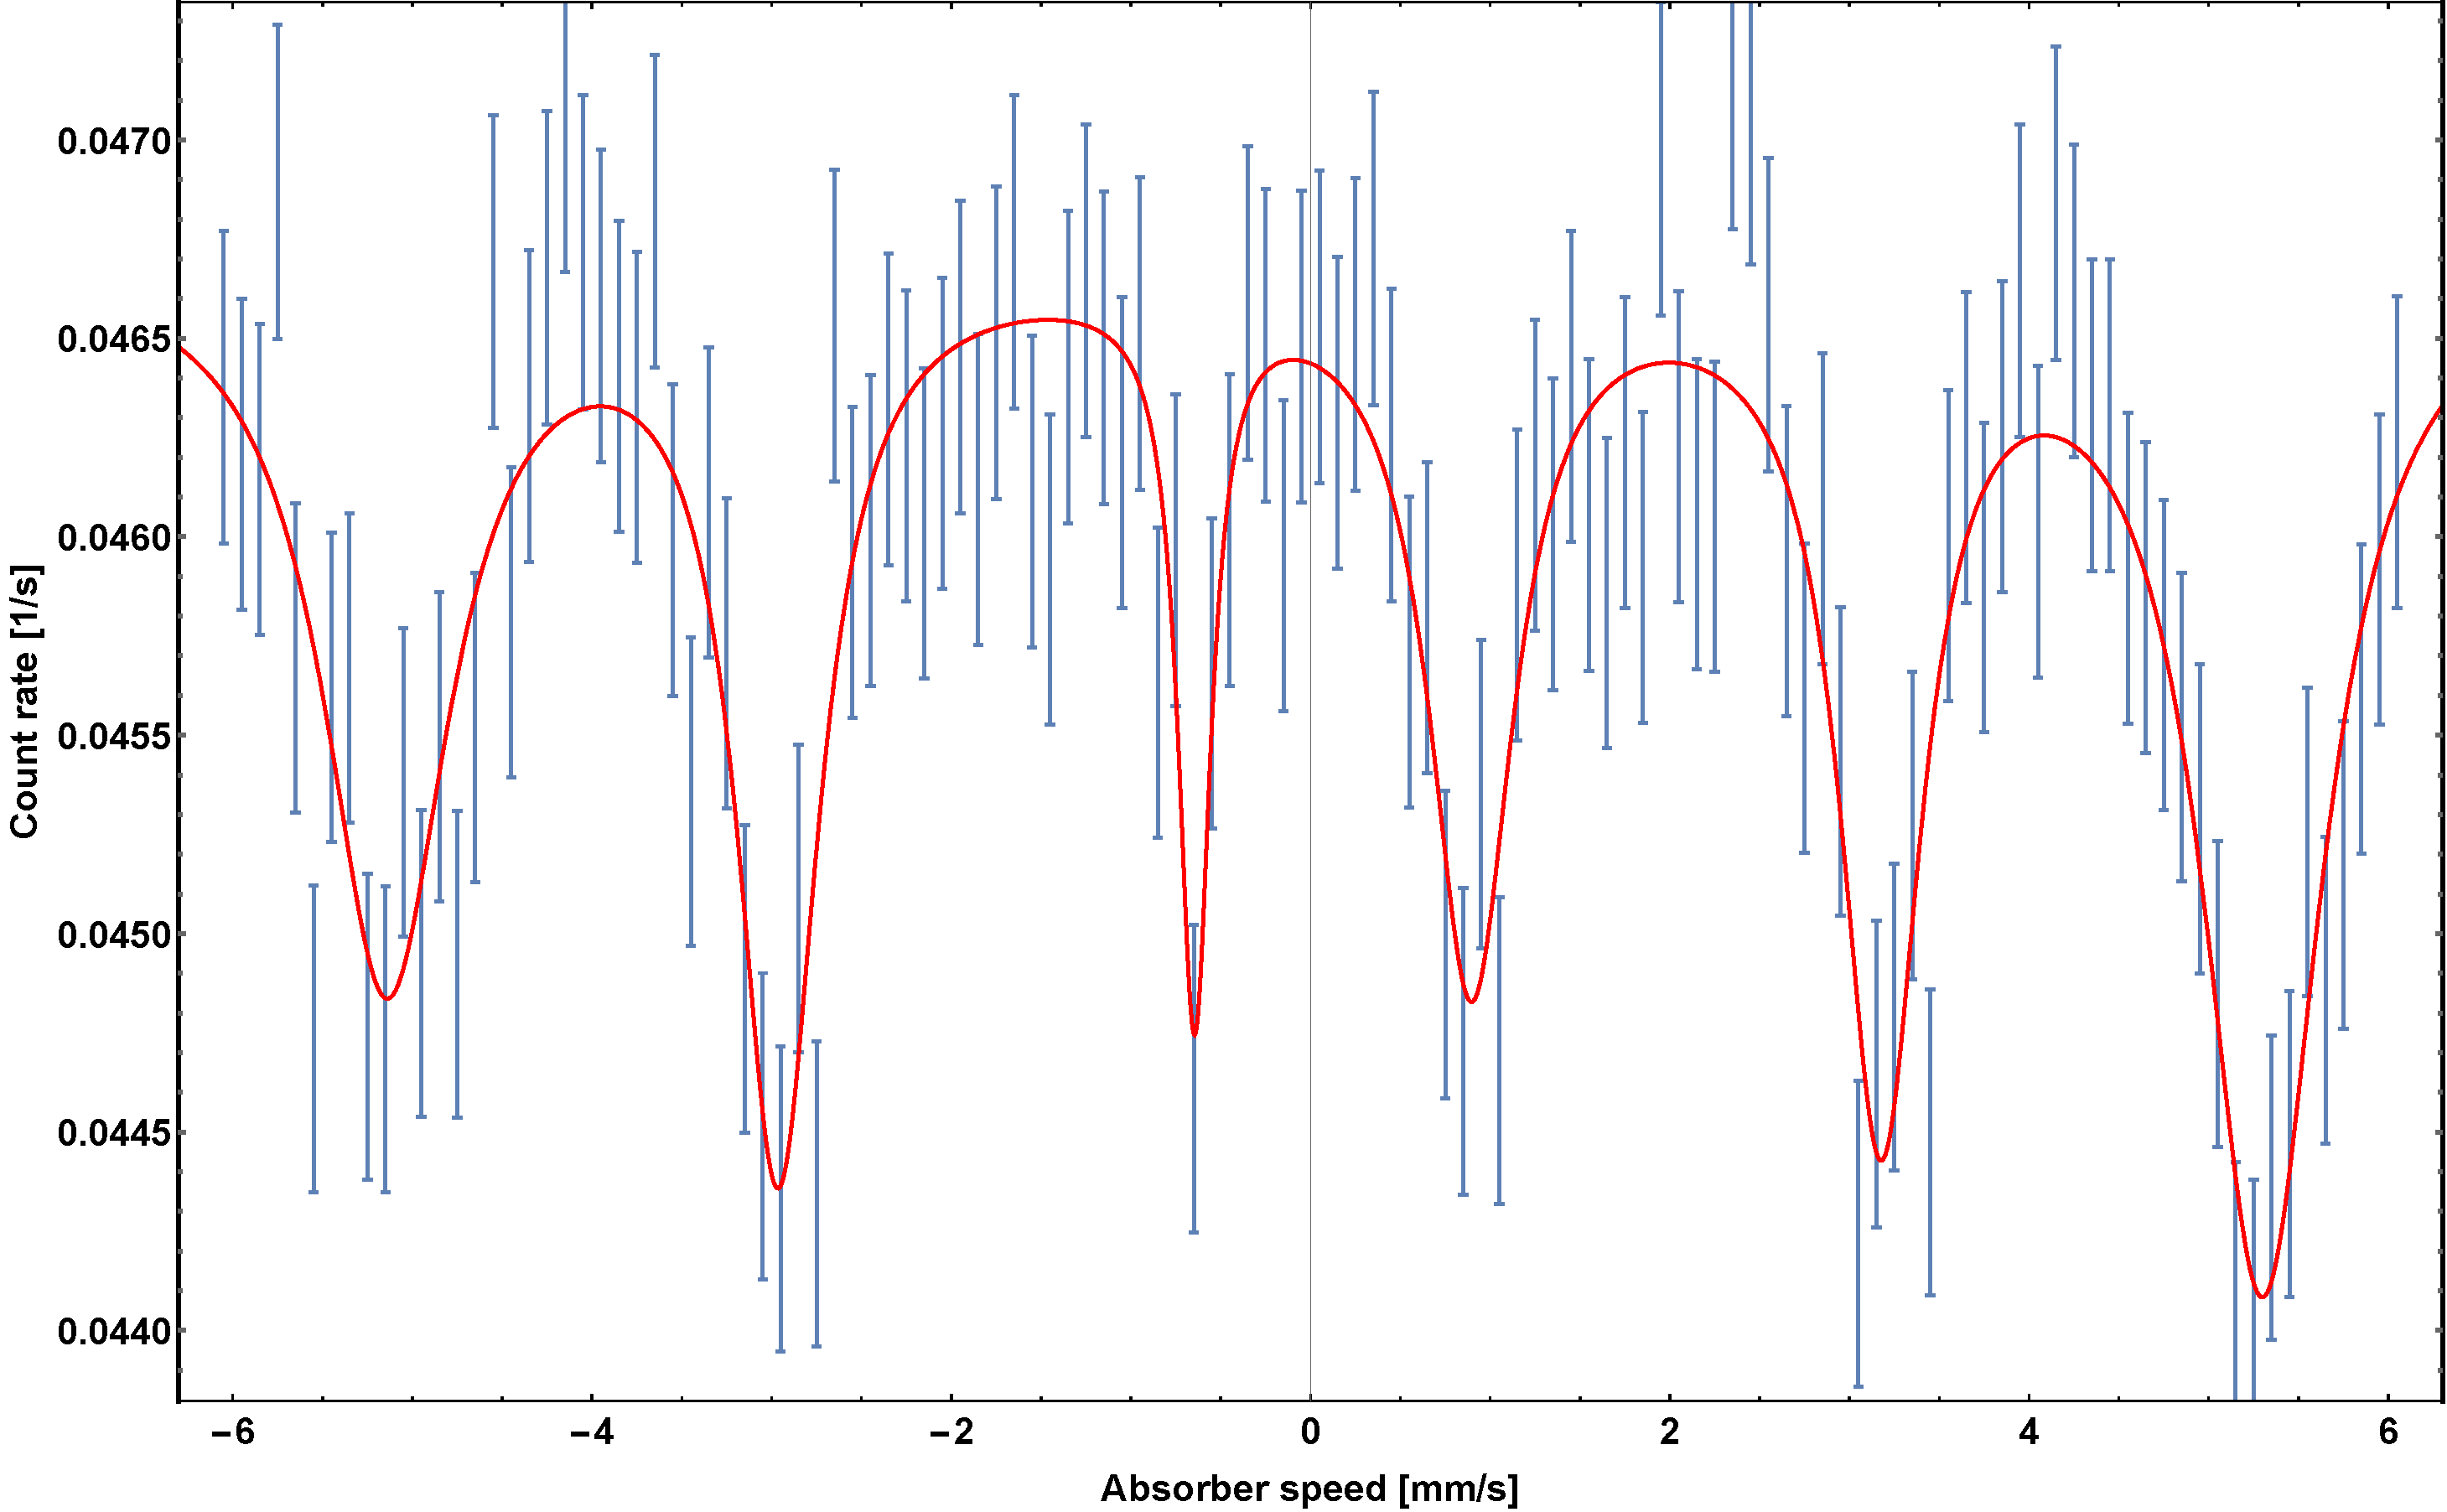
\includegraphics[width=1.0\linewidth]{graphics/natureisen}
\caption[Six-line absorber peaks]{The six-line absorber spectrum. A sum of 6 Lorentz functions was fitted to the data.}
\label{fig:natureisen}
\end{figure}
Figure \ref{fig:natureisen} shows the measurement results of the six-line absorber measurements. A sum of 6 Lorentz function, one for each peak, was fitted to the data. Gauss functions are to wide and due to the large uncertainties and the relatively low number of points per peak, the effort of doing Voigt fits is not warranted. The Lorentz fit describes the data well enough, with a $\chi^2$ value of 1.0. The peak positions and the corresponding energy shifts are listed in table \ref{tb:peakpositions}.\\
\begin{table}\centering
	\begin{tabular}{@{}lll@{}}
		\toprule
		Peak i & $v_i$ [mm/s]&$\Delta E$ [neV]\\
		\midrule
		1 & $-5.14\pm0.05$ & $-246.9\pm2.4$ \\
		2 & $-2.96\pm0.03$ & $-142.4\pm1.6$ \\
		3 & $-0.65\pm0.03$ & $-31.0\pm1.4$ \\
		4 & $0.90\pm0.04$ & $43.0\pm2.0$ \\
		5 & $3.18\pm0.03$ & $152.5\pm1.6$ \\
		6 & $5.30\pm0.03$ & $254.6\pm1.7$\\
		\bottomrule
	\end{tabular}
	\caption[Six-line absorber peak positions]{Positions of the peaks in the six-line absorber velocity spectrum.}
	\label{tb:peakpositions}
\end{table}
\subsubsection{Isomeric shift}
As the isomer shift is the offset from 0, three values can be determined here. One for the shift when comparing the first and sixth peak, on for the second and fifth and one for the third and forth. 
\begin{table}\centering
	\begin{tabular}{@{}lll@{}}
		\toprule
		Peaks & $v_{iso}$ [mm/s]&$E_{iso}$ [neV]\\
		\midrule
		6-1 & $0.08\pm0.03$ & $3.8\pm1.5$ \\
		5-2 & $0.106\pm0.023$ & $5.1\pm1.1$ \\
		4-3 & $0.125\pm0.025$ & $6.0\pm1.2$ \\
		\bottomrule
	\end{tabular}
	\caption[Six-line absorber: Isomer shift]{Isomer shifts of the six-line absorber.}
	\label{tb:isomershifts}
\end{table}
The weighted means of the values listed in table \ref{tb:isomershifts} are
\begin{align}
\overline{v}_{iso}&=\unit{(0.102\pm0.024)}{mm/s}\\
\overline{E}_{iso}&=\unit{(4.9\pm1.1)}{neV}
\end{align}
which both include their literature values $v_{iso}^{lit}=\unit{0.11}{mm/s}$ and $E_{iso}^{lit}=\unit{5.3}{neV}$ from the data sheet of the sample in their relatively large $1\sigma$ intervals.

\subsubsection{Magnetic moment}
Equation \ref{eq:HFS} yields
\begin{equation}
E_i=E_{iso}-E_{HFS}=E_{iso}-\left(\frac{\mu_em_e}{Ie}+\frac{\mu_gm_g}{I_g}\right)\cdot B
\end{equation}
which can be written using the velocities
\begin{equation}
v_i=v_{iso}-\frac{c}{E_0}\left(\frac{\mu_em_e}{Ie}+\frac{\mu_gm_g}{I_g}\right)
\end{equation}
The nuclear spins are$I_g=\nicefrac{1}{2}$ and $I_e=\nicefrac{3}{2}$. Table \ref{tb:peakqnumbers} shows the magnetic quantum numbers that correspond to the peaks.
\begin{table}\centering
	\begin{tabular}{@{}lll@{}}
		\toprule
		Peak & $m_e$&$m_g$\\
		\midrule
		1 & \nicefrac{3}{2} & \nicefrac{1}{2}\\
		2 & \nicefrac{1}{2} & \nicefrac{1}{2}\\
		3 & -\nicefrac{1}{2}& \nicefrac{1}{2}\\
		4 & \nicefrac{1}{2}& -\nicefrac{1}{2}\\
		5 & -\nicefrac{1}{2}& -\nicefrac{1}{2}\\
		6 & -\nicefrac{3}{2}& -\nicefrac{1}{2}\\
		\bottomrule
	\end{tabular}
	\caption[Quantum numbers of the peaks]{The magnetic quantum numbers corresponding to the peaks.}
	\label{tb:peakqnumbers}
\end{table}
The formulas still contain the unknown magnetic field. One can now calculate the velocity differences of the corresponding peaks
\begin{align}
\Delta v_a=v_6-v_1=\frac{2c}{E_0}&\left(\mu_g-\mu_e\right)B\\
\Delta v_b=v_5-v_2=\frac{2c}{E_0}&\left(\mu_g-\frac{\mu_e}{3}\right)B\\
\Delta v_c=v_4-v_3=\frac{2c}{E_0}&\left(\mu_g+\frac{\mu_e}{3}\right)B
\label{eq:thevaformulas}
\end{align}
With these three variables, there are three possible combinations to get formulas for the magnetic moment of the excited state. 
\begin{align}
\frac{\Delta v_a}{\Delta v_b}&=\frac{\mu_g-\mu_e}{\mu_g-\frac{\mu_e}{3}}\\
\frac{\Delta v_b}{\Delta v_c}&=\frac{\mu_g-\mu_e}{\mu_g+\frac{\mu_e}{3}}\\
\frac{\Delta v_c}{\Delta v_a}&=\frac{\mu_g+\frac{\mu_e}{3}}{\mu_g-\frac{\mu_e}{3}}
\end{align}
The magnetic moment of the ground state is given in \cite{stone} as $\mu_g=(0.09044\pm0.0007)\cdot\mu_N$, where the nuclear magneton is $\mu_N=\unit{3.152\cdot10^{-8}}{eV/T}$. Solving these separate formulas for the magnetic moment of the excited state and applying standard Gaussian error propagation yields (in units of $\mu_N$)
\begin{align}
\frac{\Delta v_a}{\Delta v_b}\Rightarrow \mu_e&=\mu_g\frac{3\Delta v_a-\Delta v_b}{\Delta v_a-3\Delta v_b}=\unit{(-0.146\pm0.005)}{\mu_N}\\
\frac{\Delta v_b}{\Delta v_c}\Rightarrow\mu_e&=3\mu_g\frac{\Delta v_c-\Delta v_b}{\Delta v_c+\Delta v_b}=\unit{(-0.162\pm0.003)}{\mu_N}\\
\frac{\Delta v_c}{\Delta v_a}\Rightarrow\mu_e&=\mu_g\frac{\Delta v_c-\Delta v_a}{\Delta v_a/3+\Delta v_c}=\unit{(-0.160\pm0.003)}{\mu_N}
\end{align}
Stone \cite{stone} lists the magnetic moment of the excited state as $\mu_e=\unit{(-0.1549\pm0.0002)}{\mu_N}$.
All values enclose this value at least in their $3\sigma$ intervals. 

\subsubsection{The magnetic field at the nucleus}
With the magnetic moments known, the magnetic fields can now be calculated from the formulas in equation \ref{eq:thevaformulas}
\begin{align}
	B_a&=\unit{(33.7\pm0.7)}{T}\\
	B_b&=\unit{(32.4\pm0.4)}{T}\\
	B_c&=\unit{(31.7\pm1.5)}{T}
\end{align}
which are all within $2\sigma$ of the literature value $B_{lit}=\unit{33}{T}$ \cite{Fultz}.


\section{Summary}
\subsection{Background}
By measuring the absorption for different thicknesses of aluminum, the background count rate was determined to be:
\begin{equation*}
A_C= (29.74\pm0.17)s^-1
\end{equation*}	
\subsection{Attenuation by the acrylic glass}
The attenuation coefficient for the acrylic glass was measured with the result:
\begin{equation*}
\mu_{acr}=\unit{(1.21\pm0.02)}{1/cm}
\end{equation*}
The value does not match the calculated one $\mu=\unit{1.31019}{1/cm}$. For the latter, nominal values for $E_\gamma$=\unit{15}{keV} were used, which is slightly higher then the energy of the iron transition. The effect of this would be lower attenuation coefficients however. Their difference can thus only be explained by different thicknesses of the glass for the absorber and the empty acrylic glass plate. A $5\%$ difference in thickness would close the gap between the values.
\subsection{Single line absorber}
The isomeric shift was measured
\begin{equation*}
E_{iso}= \unit{8.61\pm0.24\cdot10^{-9}}{eV}
\end{equation*}. 
With the calculated effective absorber thickness $T_A=(6.2\pm0.4)$, the Debye-Waller factor of the source was determined:
\begin{equation*}
f_s=0.51\pm0.08
\end{equation*}
The mean life as determined from the Voigt fit is:
\begin{equation*}
\scalebox{1.5}{$\tau$}=\unit{(195\pm140)}{ns}
\end{equation*}

\subsection{Six line absorber}
By fitting the sum of six Lorentz curves to the recorded spectrum of natural iron, the following values were determined during evaluation.
\begin{table}[H]\centering
	\begin{tabular}{@{}llllll@{}}
		\toprule
		 Quantity& Value \\
		\midrule
		$\overline{E_{iso}}$ & \unit{(4.9\pm1.1)}{neV}\\
		$\mu_ea$ & \unit{(-0.146\pm0.005)}{\mu_N} \\
		$\mu_eb$ & \unit{(-0.162\pm0.003)}{\mu_N}\\
		$\mu_ec$ & \unit{(-160\pm0.003)}{\mu_N}\\
		$B_a$ & \unit{(33.7\pm0.7)}{T}  \\
		$B_b$ & \unit{(32.4\pm0.4)}{T}  \\
		$B_c$ & \unit{(31.7\pm1.5)}{T}  \\ 
		\bottomrule
	\end{tabular}
	\caption[Summary six line absorber]{Summary of the results for the six line absorber}
	\label{tb:summary:sixline abs}
\end{table}
The isomeric shift lies within one standard deviation of the literature value $E^{lit}_{iso}=\unit{5.3}{neV}$. The measured values for the magnetic moment enclose within their 3$\sigma$ intervals the literature value $\mu_e (-0.1549\pm0.002)$ \cite{stone}.

\newpage

\begin{thebibliography}{99}
\bibitem{Wegener}
Wegener, Horst. "Der Mößbauer Effekt und seine Anwendungen". Mannheim 1966
\bibitem{Demtröder}
Demtröder, Wolfgang. Experimentalphysik 3 Atome, Moleküle und Festkörper

\bibitem{jakobs}
Jakobs, Karl. Experimentelle Methoden der Teilchenphysik. Vorlesungsskript 2014
\bibitem{Eyges}
Eyges, Leonard. Physics of the Mössbauer effect. 1965
\bibitem{anleitung}
A.Zwerger(2007), S.Winkelmann(1/2011), M.Köhli (2/2011). Versuchsanleitung Fortgeschrittenen Praktikum Teil II - Der Mößbauer-Effekt. 2012
\bibitem{khwz}
M.Köhler(8/2010), M.Köhli (4/2011). Versuchanleitung Fortgeschrittenen Praktikum Teil I - Kurze Halbwertszeiten
\bibitem{landgraf}
U.Landgraf. Eichspektrum der Americium-Quelle (1997)
\bibitem{webelements}
https://www.webelements.com/ (28.4.2016)
\bibitem{Frauenfelder}
S. Margulies, P. Debrunner, H. Frauenfelder. Transmission and line broadening in the Mössbauer effect II. 1962
\bibitem{stone}
Stone, N.J. \emph{Table of Nuclear Magnetic Dipole and Electric Quadrupole Moments.} Oxford Physics.
\bibitem{Fultz}
Fultz, Brent.\emph{Moessbauer Spectrometry in Characterization of Materials.} John Wiley. New York, 2011.
\bibitem{Olivero}
J.J.Olivero, R.L. Longbothum. Empirical fits to the voigt line width: A brief review. 1997. http://www.sciencedirect.com/science/article/pii/0022407377901613
\end{thebibliography}

\end{document}
